\documentclass{beamer}

\mode<presentation>
{
\usetheme{Madrid}
}

\usepackage{graphics, graphicx}
\usepackage{booktabs}
\DeclareGraphicsExtensions{.pdf,.png,.jpg,.gif}

\title{Linux Beginner Guide}

\author{Jaewoong Lee}

\institute[UNIST]
{
	Ulsan National Institute of Science and Technology
	\medskip
	\newline
	\textit{jwlee230@unist.ac.kr}
}

\date{\today}

\begin{document}
	\begin{frame}
		\titlepage
	\end{frame}

	\begin{frame}
		\frametitle{Introduction}
		
		In this guide, I assume that followings are already installed:
		\begin{enumerate}
			\item Ubuntu 16.04.2 or Higher
			\item ZSH 5.0.2 or Higher
			\item VIM 8.1 or Higher
			\item We will connect to server via SSH
		\end{enumerate}

		With this guide, you can use and understand Linux system. \\
		Also, this guide includes as little information about operating system as possible. If you find some fault in the strict sense of the word, that means you are not \textbf{beginner}. 
	\end{frame}

	\begin{frame}
		\frametitle{Overview}
		\tableofcontents
	\end{frame}

	\section{Linux?}
	
	\begin{frame}
		\frametitle{Linux?}
		\begin{figure}[h!]
			\centering
			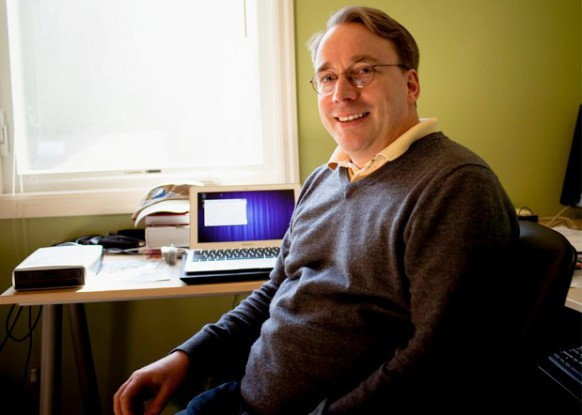
\includegraphics[width=0.4 \linewidth]{figures/linus.jpg}
			\caption{Linus Torvalds, Inventor of Linux}
		\end{figure}
	
		Linux is one of the most famous OS as Windows and macOS. \\
		Linux is open-source project. \\
		Android, OS for mobile, is based on Linux. 
	\end{frame}

	\begin{frame}
		\frametitle{Ubuntu?}
		\begin{figure}[h!]
			\centering
			
\includegraphics[width=0.3 \linewidth]{figures/ubuntu.jpg}
			\caption{Logo of Ubuntu}
		\end{figure}
		Ubuntu is an OS which is based on Linux. \\
		Ubuntu is the best OS in Linux-like OS, because of convenience of its installation and usage.
	\end{frame}
	
	\section{Basic Linux Command}
	
	\begin{frame}
		\frametitle{Where we start}
		\begin{figure}[h!]
			\centering
			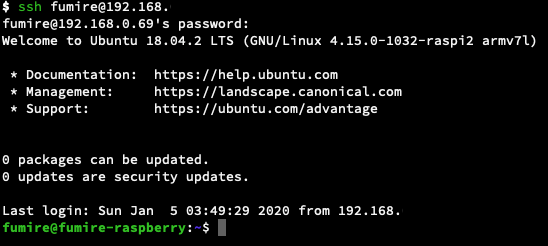
\includegraphics[width=0.5 \linewidth]{figures/1.png}
			\caption{Here is where we start}
		\end{figure}
	
		After you connect to server via SSH, you can see like this. \\
		Here is where we start! \\
		\textit{fumire} will be user name, and \textit{fumire-raspberry} will be server name. 
	\end{frame}

	\begin{frame}
		\frametitle{pwd}
		\begin{figure}[h!]
			\centering
			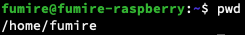
\includegraphics[width=0.5 \linewidth]{figures/2.png}
			\caption{Result of \textit{pwd} Command}
		\end{figure}
		\textit{pwd} is abbr. of "Print Working Directory". \\
		You can see where you are with \textit{pwd} command. \\
		Also, "/home/username" is your \textit{home folder}, a.k.a. '$\sim$'.
	\end{frame}

	\begin{frame}
		\frametitle{ls}
		\begin{figure}[h!]
			\centering
			
\includegraphics[width=0.7 \linewidth]{figures/3.png}
			\caption{Result of \textit{ls} Command}
		\end{figure}
	
		\textit{ls} stands for "List". \\
		\textit{ls} command lists current directory contents. \\
		If current directory is empty, the result will be nothing. 
	\end{frame}

	\begin{frame}
		\frametitle{Configuration}
		However, you have not completed configuration. Therefore, finish settings with following command:
		\begin{example}
			\$ git clone https://github.com/Fumire/.dotfiles.git \\
			\$ cd .dotfiles \\
			\$ make \\
			\$ chsh -s /usr/bin/zsh
		\end{example}
		Note that you should input command only after '\$'. \\
		After executing commands, you should restart your shell. 
	\end{frame}

	\begin{frame}
		\frametitle{Configuration \textit{(Cont.)}}
		\begin{figure}[h!]
			\centering
			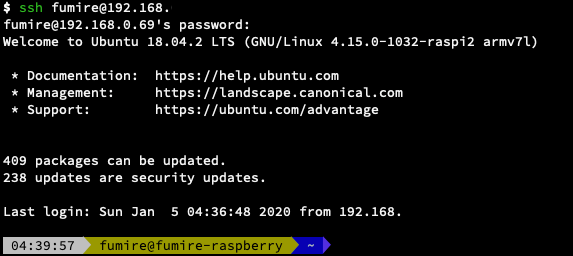
\includegraphics[width=0.7 \linewidth]{figures/4.png}
			\caption{ZSH}
		\end{figure}
	
		With successful configuration, you can see like this. 
	\end{frame}

	\begin{frame}
		\frametitle{Tip!}
		\begin{figure}[h!]
			\centering
			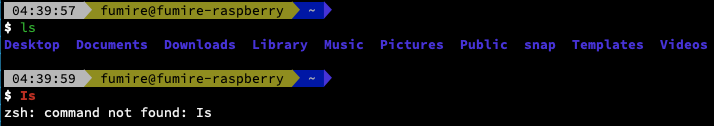
\includegraphics[width=0.7 \linewidth]{figures/5.png}
			\caption{Right Command vs. Wrong Command}
		\end{figure}
		
		You can easily know this command is right with ZSH as figure.  
	\end{frame}

	\begin{frame}
		\frametitle{mkdir}
		\textit{mkdir} stands for "Make Directory". \\
		You can make a directory which named 'test' as following: 
		\begin{example}
			\$ mkdir test \\
			or \\
			\$ md test \\
		\end{example}
		\textit{mkdir} returns nothing. Literally, \textit{mkdir} command only make directory. \\
		You can check that the directory has been made with \textit{ls} command. 
	\end{frame}

	\begin{frame}
		\frametitle{cd}
		\textit{cd} is abbr. of "Change Directory". \\
		You can change your working directory to 'test' as following:
		\begin{example}
			\$ pwd \\
			\$ cd test\\
			\$ pwd \\
		\end{example}
	
		Also, you can go your home folder at once with \textit{cd}, no matter where you are.
		\begin{figure}[h!]
			\centering
			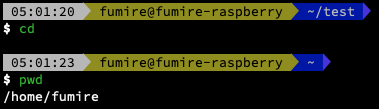
\includegraphics[width=0.7 \linewidth]{figures/6.png}
			\caption{\textit{cd} will guide you to home folder}
		\end{figure}
	\end{frame}

	\begin{frame}
		\frametitle{Tip!}
		If you hit "Tab" button, ZSH will give proper candidates. \\
		Following example shows what ZSH gives.
		\begin{figure}
			\centering
			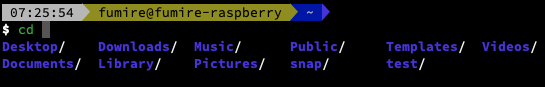
\includegraphics[width=0.7 \linewidth]{figures/10.png}
			\caption{Shortcut with Tab}
		\end{figure}
	\end{frame}

	\begin{frame}
		\frametitle{man and -$ $-help}
		You can get detailed information about command as following:
		\begin{example}
			\$ man ls \\
			and/or \\
			\$ ls -$ $-help
		\end{example}
		This guide will give simple information about Linux command. Hence, when you have curiosity about command, use these command.
	\end{frame}

	\begin{frame}
		\frametitle{Directory Structure}
		Try following commands:
		\begin{example}
			\$ cd test\\
			\$ ls -al
		\end{example}
		Then, you can see like this:
		\begin{figure}[h!]
			\centering
			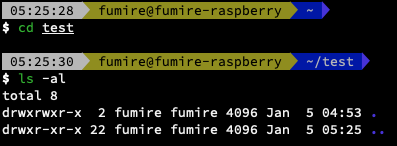
\includegraphics[width=0.3 \linewidth]{figures/7.png}
			\caption{Result of \textit{ls} command}
		\end{figure}
		All directory has '.' and '..', even though the directory is empty. \\
		'.' means current directory itself; and, '..' means parent directory.
	\end{frame}

	\begin{frame}
		\frametitle{touch}
		\textit{touch} command make new file or touch the file.
		
		Try following example:
		\begin{example}
			\$ cd \\
			\$ touch t \\
			\$ ls
		\end{example}
		
		Then, you can see that the file which name 't' has been made. 
	
		\begin{figure}[h!]
			\centering
			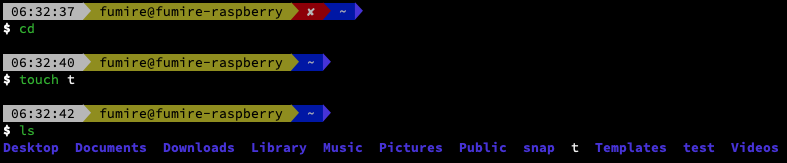
\includegraphics[width=0.5 \linewidth]{figures/8.png}
			\caption{Result of \textit{touch} Command}
		\end{figure}
	\end{frame}

	\begin{frame}
		\frametitle{mv}
		\textit{mv} command moves/renames file. \textit{mv} is used as:
		\begin{example}
			\$ mv SRC(source) DST(destination)
		\end{example}
		
		Try following commands: 
		\begin{example}
			\$ mv t tmp \\
			\$ ls \\
			\$ mv tmp test/ \\
			\$ ls
		\end{example}
	
		Then, you will realize that the file 'tmp' is gone. I hope that you already know where the file goes. :)
	\end{frame}

	\begin{frame}
		\frametitle{cp}
		\textit{cp} command copies SRC to DST. \textit{cp} is used as:
		\begin{example}
			\$ cp SRC DST
		\end{example}
	
		Try following commands:
		\begin{example}
			\$ cd $\sim$/test/ \\
			\$ ls \\
			\$ cp tmp tmp2 \\
			\$ ls
		\end{example}
		Then, you can realize that a new file 'tmp2' has been made. 
	\end{frame}

	\begin{frame}
		\frametitle{rm}
		\textit{rm} stands for 'Remove'. As its name, you can delete files or directory.
		\begin{example}
			\$ rm tmp2
		\end{example}
	
		When you want delete directory, use '-r' option:
		\begin{example}
			\$ rm -r directoryname
		\end{example}
	
		There is no way to restore removed files!! Beware what you remove!!
	\end{frame}

	\begin{frame}
		\frametitle{sudo}
		\textit{sudo} is abbr. of "Substitute User do"; but, many people know as "Super User do". \\

		\textit{sudo} allows a system administrator to delegate authority to give certain user the ability to run some command as another user.
		
		\begin{figure}[h!]
			\centering
			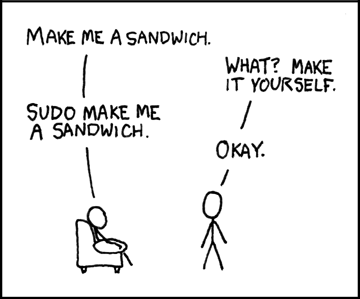
\includegraphics[width=0.3 \linewidth]{figures/sudo.png}
			\caption{XKCD: Sandwich}
		\end{figure}
	
		THINK what will happen after \textit{sudo} command!!
	\end{frame}

	\section{Edit File with VIM} 
	
	\begin{frame}
		\frametitle{Editor}
		There are three major editors in Linux.
		\begin{figure}[h!]
			\centering
			
\includegraphics[width=0.7 \linewidth]{figures/editor.png}
			\caption{Descriptions of Editor}
		\end{figure}
		For this reason, this guide use VIM editor. 
	\end{frame}

	\begin{frame}
		\frametitle{Editor \textit{Cont.}}
		\begin{figure}[h!]
			\centering
			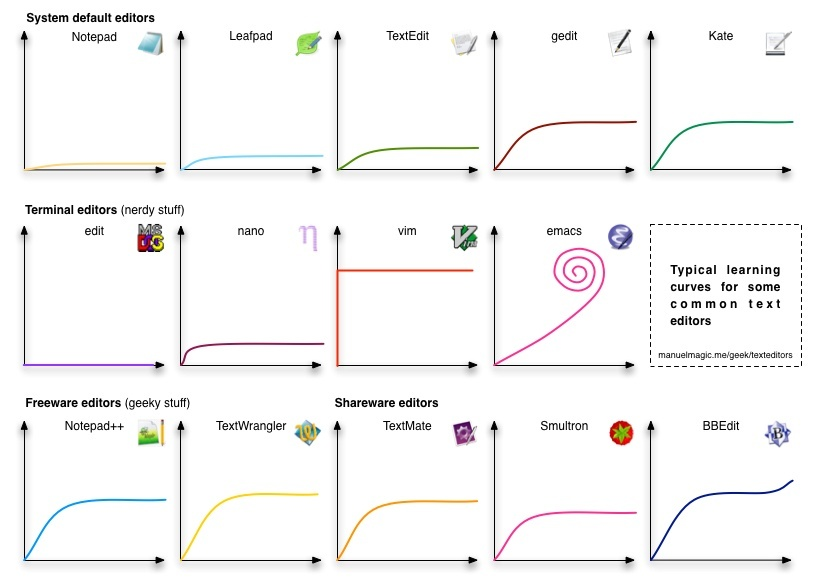
\includegraphics[width=0.7 \linewidth]{figures/curves.jpg}
			\caption{Learning Curves among Editors}
		\end{figure}
	\end{frame}

	\begin{frame}
		\frametitle{First Meet with VIM}
		With these commands, you can make/edit file.
		\begin{example}
			\$ vi tmp
		\end{example}
	
		If it is first time to open VIM, then you will see like this. 
		\begin{figure}[h!]
			\centering
			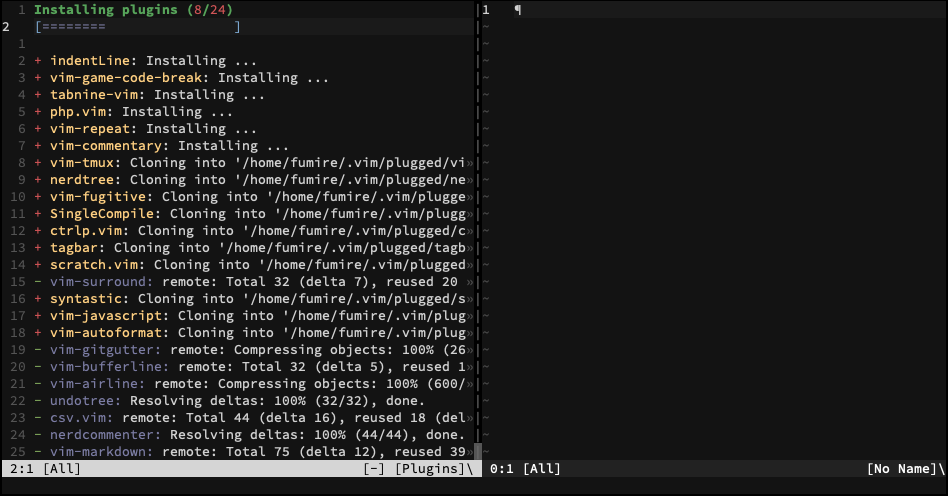
\includegraphics[width=0.5 \linewidth]{figures/9.png}
			\caption{First Time of VIM}
		\end{figure}
	\end{frame}

	\begin{frame}
		\frametitle{Modes of VIM}
		\begin{figure}[h!]
			\centering
			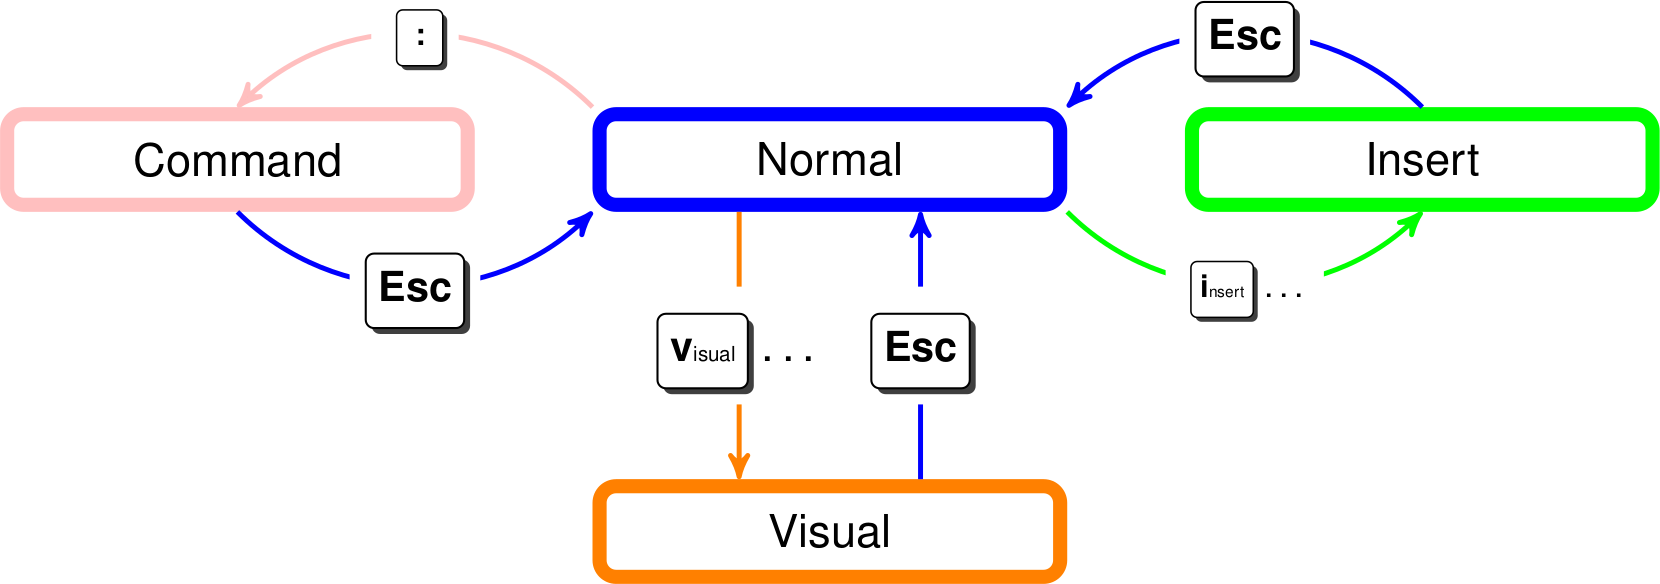
\includegraphics[width=0.7 \linewidth]{figures/modes.png}
			\caption{Three Modes in VIM}
		\end{figure}
	\end{frame}

	\begin{frame}
		\frametitle{How to Edit with VIM}
		Editing with VIM is following such steps:
		\begin{enumerate}
			\item Press 'i'
			\item Edit the file
			\item Press 'ESC'
			\item Enter ':w' which means \textit{write}
			\item Enter ':q' wihch means \textit{quit}
		\end{enumerate}
	\end{frame}

	\begin{frame}
		\frametitle{Plugin Setting (Optional)}
		You might see the error message because the plugin setting is not completed. To solve this, use following commands:
		\begin{example}
			\$ cd $\sim$/.vim/plugged/tabnine-vim/ \\
			\$ python3 install.py 
		\end{example}
		Then, all plugin acts properly without errors. 
	\end{frame}

	\section{IO Redirections}
	
	\begin{frame}
		\frametitle{cat}
		\textit{cat} stands for con\textbf{cat}enate. \textit{cat} command reads files, and writing them to standard output. \\
		Consider following example:
		\begin{example}
			\$ cd $\sim$/test/ \\
			\$ cat tmp 
		\end{example}
		You can see contents of file. 
	\end{frame}

	\begin{frame}
		\frametitle{Input/Output to file}
		If you want redirect output to file, use following example:
		\begin{example}
			\$ cat tmp $>$ output
		\end{example}
		However, this method \textit{overwrites} the contents of file. \\
		If you want preserve the file contents, use following: 
		\begin{example}
			\$ cat tmp $>>$ output
		\end{example}
	
		Also, $<$ means input from file.
	\end{frame}

	\begin{frame}
		\frametitle{Output to file \textit{Cont.}}
		In some cases, you should divide standard output and standard error. \\
		In these cases, use following commands:
		\begin{example}
			\$ commands 1$>$ STDOUT 2$>$ STDERR
		\end{example}
	
		\begin{example}
			\$ cat tmp 1$>$ ex.stdout 2$>$ ex.stderr 
		\end{example}
	\end{frame}

	\begin{frame}
		\frametitle{more / less}
		\textit{more} and \textit{less} are commands for seeing the contents of file.
		Consider following examples:
		\begin{example}
			\$ more tmp
		\end{example}
	
		\begin{example}
			\$ less tmp
		\end{example}
	\end{frame}

	\begin{frame}
		\frametitle{Pipe}
		Use pipe ($|$) to indicate input as output of previous command.
		\begin{example}
			\$ command1 $|$ command2
		\end{example}
		The output of command 1 will be the input of command2. \\
		Consider following example: 
		\begin{example}
			\$ cat tmp $|$ less
		\end{example}
	\end{frame}
	
	\section{How to Download from Web}
	
	\begin{frame}
		\frametitle{Two Ways for Download}
		There are two main ways for download.
		\begin{enumerate}
			\item curl
			\item wget
		\end{enumerate}
	\end{frame}

	\begin{frame}
		\frametitle{curl}
		\begin{example}
			\$ curl https://www.naver.com
		\end{example}
		\textit{curl} returns to standard output. If you want to get file, consider following:
		\begin{example}
			\$ curl https://www.naver.com -o naver.html
		\end{example}
	\end{frame}

	\begin{frame}
		\frametitle{wget}
		\textit{wget} returns a downloaded file as output. 
		\begin{example}
			\$ wget https://www.naver.com \\
			\$ ls
		\end{example}
	\end{frame}

	\begin{frame}
		\frametitle{gzip}
		\textit{gzip} is used for file compression and decompression.
		
		When compressing:
		\begin{example}
			\$ gzip tmp
		\end{example}
	
		When decompressing:
		\begin{example}
			\$ gzip -d tmp.gz
		\end{example}
	
		However, the examples hereinabove delete the original files. If you want \textit{keep} original file, consider following:
		\begin{example}
			\$ gzip -k tmp
		\end{example}
	\end{frame}

	\begin{frame}
		\frametitle{TAR Files}
		\textit{TAR} stands for "Tape Archives". \\
		Originally, it is used for tape; but, in nowadays, it is used for file archiving system. Usually, make a directory to one TAR files. \\
		TAR.GZ file is commonly used for distribution some software. For example:
		\begin{example}
			\$ wget https://www.python.org/ftp/python/3.8.1/Python-3.8.1.tgz
		\end{example}
		(TGZ is for TAR.GZ)
	\end{frame}

	\begin{frame}
		\frametitle{TAR Files \textit{(Cont.)}}
		You might think decompress TGZ file and make a directory from TAR file. However, you can decompress TGZ file at once:
		\begin{example}
			\$ tar -zxvf Python-3.8.1.tgz
		\end{example}
		Then, you can see the directory named 'Python-3.8.1".
	\end{frame}
	
	\section{User Permissions}
	
	\begin{frame}
		\frametitle{Permissions}
		With the following command, we can know how permissions are set:
		\begin{example}
			\$ ls -al
		\end{example}
	
		\begin{figure}[h!]
			\centering
			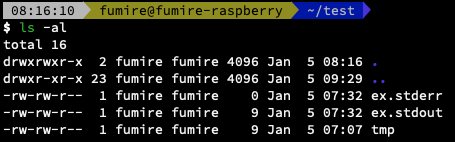
\includegraphics[width=0.4 \linewidth]{figures/11.png}
			\caption{File Permissions}
		\end{figure}
	
		The way to read this result is following:
		\begin{figure}[h!]
			\centering
			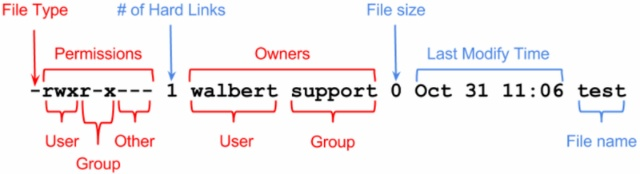
\includegraphics[width=0.5 \linewidth]{figures/permissions.jpg}
			\caption{How to Read Permissions}
		\end{figure}
	\end{frame}

	\begin{frame}
		\frametitle{chmod}
		\textit{chmod} stands for "Change Mode". You can modify permissions of files.
		
		Before input command, you should calculate simple arithmetic:
		\begin{figure}[h!]
			\centering
			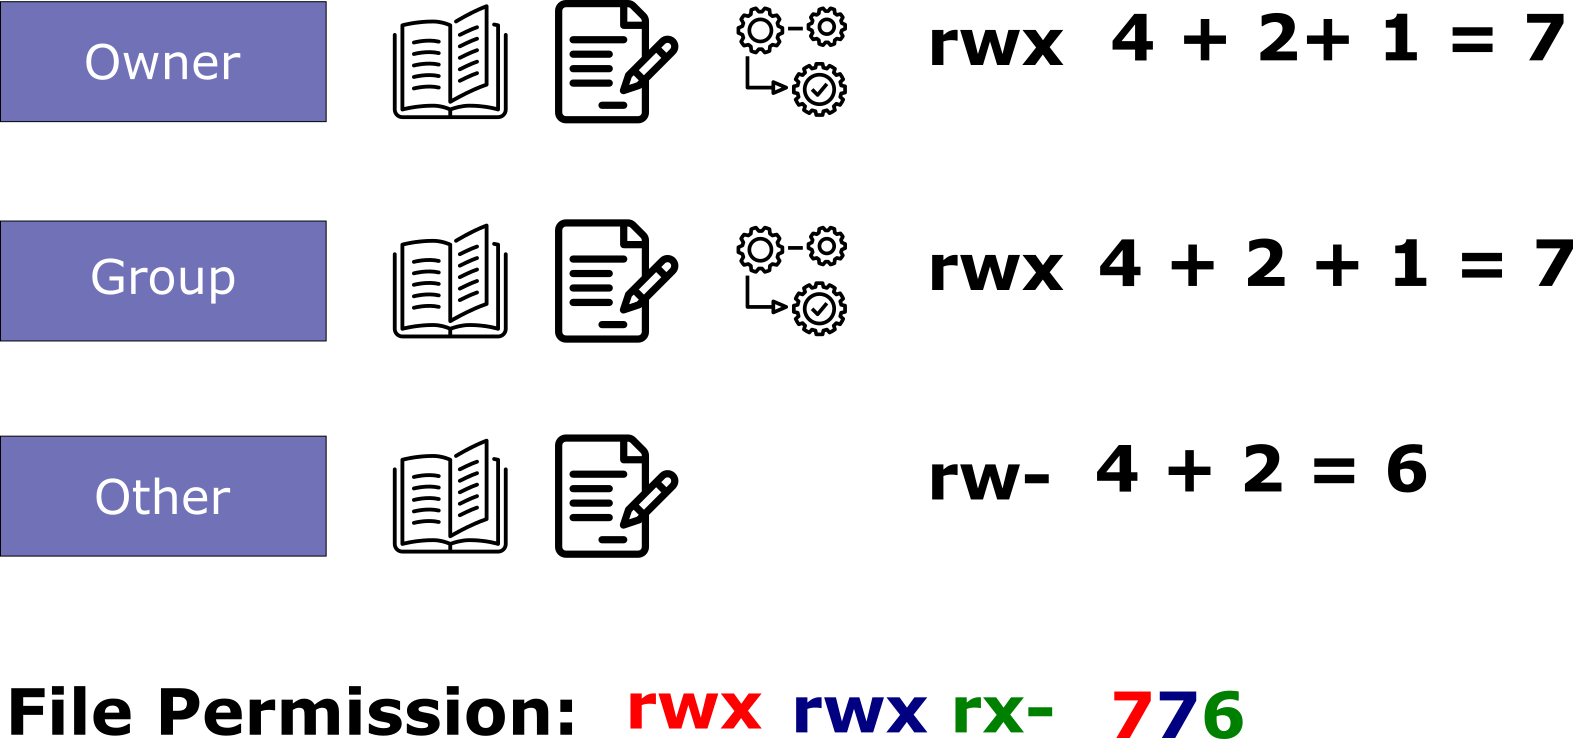
\includegraphics[width=0.4 \linewidth]{figures/permissions2.png}
			\caption{Simple Arithmetic}
		\end{figure}
		Then, you will get three digits for permission. Moreover, 660 or 770 are usually used. 
	
		\begin{example}
			\$ chmod three\_digits filename
		\end{example}
	\end{frame}

	\begin{frame}
		\frametitle{chmod \textit{(Cont.)}}
		Or, you can do as followings:
		
		\begin{example}
			\$ chmod rwx-$ $-$ $-$ $-$ $-$ $- tmp
		\end{example}
	
		\begin{example}
			\$ chmod g=rwx tmp
		\end{example}
	
		\begin{example}
			\$ chmod +x tmp
		\end{example}
	\end{frame}

	\begin{frame}
		\frametitle{chown}
		\textit{chown} stands for "change ownership". As its name, you can modify ownership of file.
		
		When you want to change only USER:
		\begin{example}
			\$ chown USER tmp
		\end{example}
	
		When you want to change both USER and GROUP:
		\begin{example}
			\$ chown USER:GROUP tmp
		\end{example}
	\end{frame}
	
	\section{Process Control}
	
	\begin{frame}
		\frametitle{Ctrl-C}
		When you have started command, but you realize that you should stop the command, then use "Ctrl-C".
		\begin{example}
			\$ sleep 99999 \\
			\$ \^{}C
		\end{example}
	
		Ctrl-C sends SIGINT, which stands for "Signal Interruption"; and, the process is going to terminate after receiving SIGINT.
	\end{frame}
	
	\begin{frame}
		\frametitle{\&}
		Consider long-time procedure, such as:
		\begin{example}
			\$ sleep 99999
		\end{example}
	
		However, with '\&', you do not have to wait procedure.
		\begin{example}
			\$ sleep 99999 \&
		\end{example}
		Then, the process is executing on background. 
	\end{frame}

	\begin{frame}
		\frametitle{jobs}
		\textit{jobs} commands shows the background process.
		\begin{example}
			\$ jobs
		\end{example}
	
		\begin{figure}[h!]
			\centering
			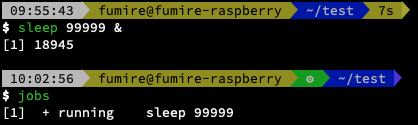
\includegraphics[width=0.5 \linewidth]{figures/12.png}
			\caption{Result of \textit{jobs}}
		\end{figure}
		You use record the [number] for handle the process. \\
	\end{frame}

	\begin{frame}
		\frametitle{kill}
		\textit{kill} command kills the process. 
		
		When you want to kill background process, consider following:
		\begin{example}
			\$ kill \%number
		\end{example}
		The number is from the \textit{jobs} command. 
		
		\begin{example}
			\$ kill process\_number
		\end{example}
		You can kill as above when you know exact process number (PID). 
	\end{frame}

	\begin{frame}
		\frametitle{nohup}
		When you lost from SSH connection, all executing process receive SIGHUP, which stands for Signal Hangup, and will be terminate even they runs on background. \\
		To prevent SIGHUP, use \textit{nohup} command. 
		
		\begin{example}
			\$ nohup sleep 99999 \&
		\end{example}
	
		However, \textit{nohup} command makes 'nohup.out' automatically. You can change output file name with IO redirection. 
	\end{frame}

	\begin{frame}
		\frametitle{screen}
		\textit{screen} prevents unintentional connection lost. 
		
		Make screen session with simple command:
		\begin{example}
			\$ screen
		\end{example}
	
		When you want to detach the screen session, use following, instead of \textit{exit}:
		\begin{example}
			\$ \^{}a, d
		\end{example}
	
		When you restore the screen session, use following command:
		\begin{example}
			\$ screen -r
		\end{example}
	\end{frame}
	
	\section{Process Control with SGE}
	
	\begin{frame}
		\frametitle{Sun Grid Engine (SGE)}
		
		\begin{figure}[h!]
			\centering
			
\includegraphics[width=0.5 \linewidth]{figures/SGE.png}
			\caption{Sun Grid Engine}
		\end{figure}
		
		We use server, not dedicated machine. Therefore, all resources should be distributed with all users. \\
		SGE can be a solution for distribution of resources. 
	\end{frame}

	\begin{frame}
		\frametitle{Script File}
		Script file is a text file containing a collection of SHELL statements. 
		
		Make a script file via VIM as:
		\begin{example}
			\$ vi tmp.sh
		\end{example}
	
		Also, the file contents should be:
		\begin{example}
			sleep 99999
		\end{example}
	
		You can execute the script file as:
		\begin{example}
			\$ sh tmp.sh
		\end{example}
	\end{frame}

	\begin{frame}
		\frametitle{qsub}
		You can submit the script file for execute with \textit{qsub} command:
		\begin{example}
			\$ qsub tmp.sh
		\end{example}
	
		When you want to designate the log file names, consider following:
		\begin{example}
			\$ qsub -e errorlog -o outputlog tmp.sh
		\end{example}
	\end{frame}

	\begin{frame}
		\frametitle{qstat}
		You can check your jobs with \textit{qstat} command:
		\begin{example}
			\$ qstat
		\end{example}
	
		If you want to check jobs from all users, consider following:
		\begin{example}
			\$ qstat -u "*"
		\end{example}
	
		Note that you should record job-ID for further handling.
	\end{frame}

	\begin{frame}
		\frametitle{qdel}
		If you want to delete submitted jobs, you can use \textit{qdel} command:
		\begin{example}
			\$ qdel job-ID
		\end{example}
	
		If you want to delete all jobs from you, consider following:
		\begin{example}
			\$ qdel -u "username"
		\end{example}
	\end{frame}

\end{document}